\documentclass{article}
\usepackage{enumerate}
\usepackage{amsmath}
\usepackage{amssymb}
\usepackage{graphicx}
\usepackage{subfigure}
\usepackage{geometry}
\def\degree{${}^{\circ}$}
\geometry{left=3.0cm,right=3.0cm,top=3.0cm,bottom=3.0cm}
\begin{document}

\section*{Problem 1.}
	\begin{enumerate}[(a)]
	\item
	$$(\omega_0^2-\omega_{dr}^2)^2+\left(\frac{b\omega_{dr}}{m}\right)^2=\omega_{dr}^4-\left(2\omega_0^2-\frac{b^2}{m^2}\right)\omega_{dr}^2+\omega_0^4$$
	When $\omega_{dr}^2=\omega_0^2-\frac{b^2}{2m^2}$, it get its minimum value
	$$\omega_{dr}=\omega_{res}=\sqrt{\omega_0^2-\frac{b^2}{2m^2}}$$
	$$A(\omega_{res})=\frac{F_0}{b\sqrt{\omega_0^2-\frac{b^2}{4m^2}}}$$
	\item
	\begin{align*}
	(\omega_0^2-\omega_{dr}^2)^2+\left(\frac{b\omega_{dr}}{m}\right)^2&=(\omega_0-\omega_{dr})^2(\omega_0+\omega_{dr})^2+\left(\frac{b\omega_{dr}}{m}\right)^2\\
	&\approx 4\omega_0^2(\omega_0-\omega_{dr})^2+\omega_0^2\frac{b^2}{m^2}\\
	&=(2\omega_0)^2\left[(\omega_0-\omega_{dr})^2+\frac{b^2}{4m^2}\right]
	\end{align*}
	$$A(\omega_{dr})\approx \frac{F_0}{2m\omega_0\sqrt{(\omega_0-\omega_{dr})^2+\frac{b^2}{4m^2}}}$$
	\begin{figure}[h!]
		\centering				
		\subfigure[$F_0=1,m=1,\omega_0=1,b=1$]{
		\label{Fig.sub.1}
		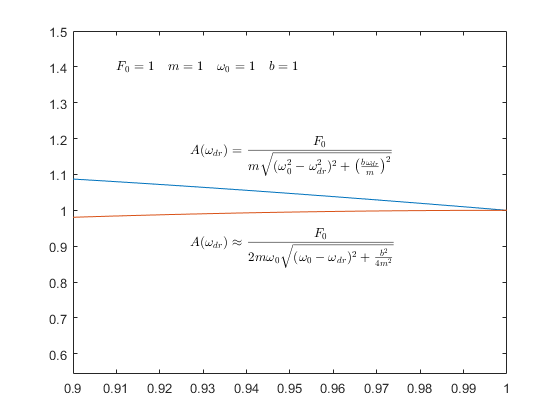
\includegraphics[width=5cm]{p1.png}}
		\subfigure[$F_0=3,m=1,\omega_0=1,b=1$]{
		\label{Fig.sub.2}
		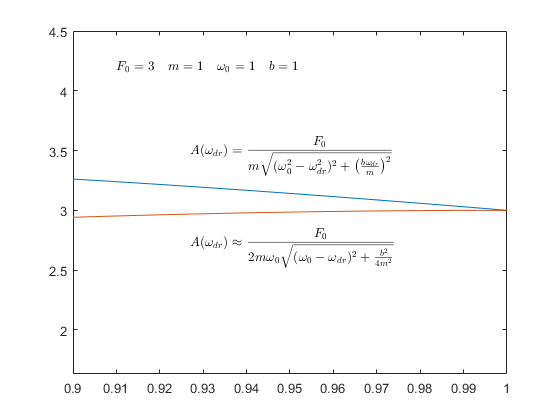
\includegraphics[width=5cm]{p1_a.png}}
		\subfigure[$F_0=1,m=3,\omega_0=1,b=1$]{
		\label{Fig.sub.3}
		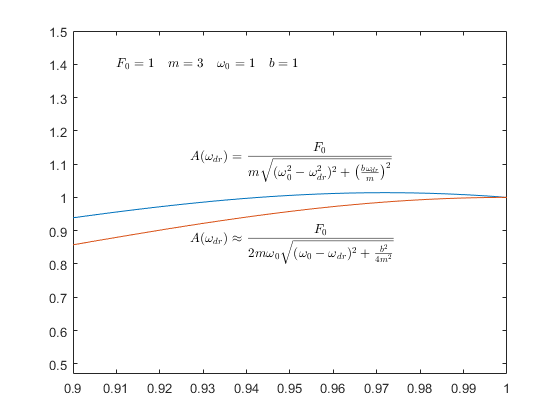
\includegraphics[width=5cm]{p1_b.png}}
		\subfigure[$F_0=1,m=1,\omega_0=3,b=1$]{
		\label{Fig.sub.4}
		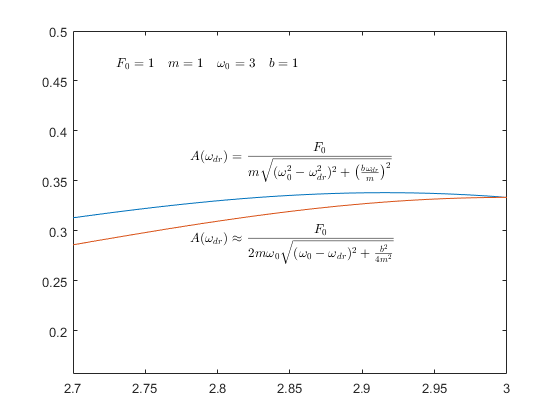
\includegraphics[width=5cm]{p1_c.png}}
		\subfigure[$F_0=1,m=1,\omega_0=1,b=3$]{
		\label{Fig.sub.5}
		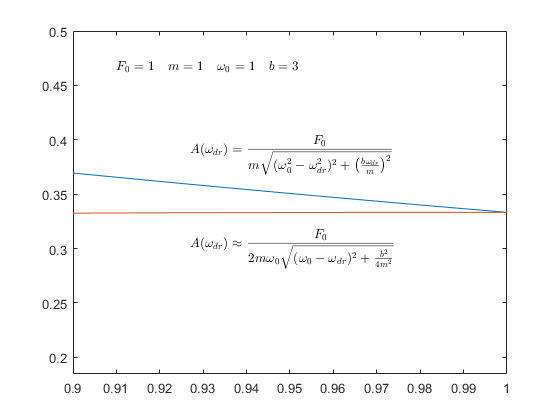
\includegraphics[width=5cm]{p1_d.png}}
		\caption{The exact and approximate curve}
		\label{figure}
	\end{figure}
	\item
	Since $\Delta\omega_{dr}$ and $\frac{b}{m}$ is small, $\omega_{dr}\approx\omega_{res}\approx\omega_0$
	$$A(\omega_{dr})=\frac{\sqrt{2}}{2}A(\omega_{res})
	=\frac{\sqrt{2}F_0}{2b\sqrt{\omega_0^2-\frac{b^2}{4m^2}}}
	\approx\frac{F_0}{\sqrt{2}b\omega_0}$$
	$$A(\omega_{dr})=\frac{F_0}{m\sqrt{(\omega_0^2-\omega_{dr}^2)^2+\left(\frac{b\omega_{dr}}{m}\right)^2}}
	=\frac{F_0}{m\sqrt{(\omega_0-\omega_{dr})^2(\omega_0+\omega_{dr})^2+\frac{b^2\omega_0^2}{m^2}}}
	\approx\frac{F_0}{m\sqrt{\omega_0^2\Delta\omega_{dr}^2+\frac{b^2\omega_0^2}{m^2}}}$$
	$$2b^2\omega_0^2
	=m^2\left(\omega_0^2\Delta\omega_{dr}^2+\frac{b^2\omega_0^2}{m^2}\right)$$
	$$\Delta\omega_0=\frac{b}{m}$$
	\end{enumerate}		

\section*{Problem 2.}
\begin{enumerate}[(a)]
	\item
	$$\tan\varphi=\frac{b\omega_{dr}}{m(\omega_{dr}^2-\omega_0^2)}=-1$$
	$$4\omega_{dr}=\omega_0^2-\omega_{dr}^2$$
	$$\omega_{dr}=\sqrt{4+\omega_0^2}-2$$
	\item
	$$\frac{F_0}{m\sqrt{(\omega_0^2-\omega_1^2)^2+\left(\frac{b\Omega_1}{m}\right)^2}}
	=\frac{F_0}{m\sqrt{(\omega_0^2-\Omega_2^2)^2+\left(\frac{b\Omega_2}{m}\right)^2}}$$
	$$\omega_0^4-2\omega_0^2\Omega_1^2+\Omega_1^4+\frac{b^2\Omega_1^2}{m^2}
	=\omega_0^4-2\omega_0^2\Omega_2^2+\Omega_2^4+\frac{b^2\Omega_2^2}{m^2}$$
	$$\omega_0=\sqrt{\frac{\Omega_1^2+\Omega_2^2}{2}+\frac{b^2}{2m^2}}$$
\end{enumerate}

\section*{Problem 3.}
	Solved in a FOR whose x-axis is the perpendicular to the slide and y-axis is opposite to the motion direction.
	$$a'=a=g\sin\alpha-\mu g\cos\theta$$
	Obviously, in this frame of reference, the surface of the liquid in the container should be perpendicular to the direction of the acceleration.\\
	On the direction of x-axis, $$a_x=a'-g\sin\theta=-\mu g\cos\theta$$
	On the direction of y-axis, $$a_y=g\cos\theta$$
	So the angle between $a$ and y-axis equals $\arctan\mu$, which is the angle that the surface of the liquid in the container forms with the inclined plane.
	
\section*{Problem 4.}
\begin{enumerate}
	\item
	Solved in the FOR of ground.\\
	No, it doesn't change.\\
	$$F=-(k_1+k_2)\Delta l$$
	$$T=2\pi\sqrt{\frac{m}{k_1+k_2}}$$
	\item
	Solved in the FOR of the elevator.\\
	Yes, it changes.
	$$mg=(k_1+k_2)(l_1-l_0)$$
	$$m(g-a)=(k_1+k_2)(l_2-l_0)$$
	$$\Delta l=l_1-l_2=\frac{ma}{k_1+k_2}$$
\end{enumerate}

\section*{Problem 5.}
The direction of the angular acceleration vector is to the central axis of the rotation of the earth.\\
The observer on the equator will find himself moving at a speed while another won't.

\section*{Problem 6.}
Let the horizontal distance between the center and the object be x, all of the points in the domain of x remain at rest
\begin{enumerate}[(a)]
	\item
	$$\tan\theta=y'=\alpha x$$
	$$\mu_smg\cos\theta\geqslant mg\sin\theta$$
	$$\tan\theta\leqslant\mu_s$$
	$$x\leqslant\frac{\mu_s}{\alpha}$$
	\item
	Solved in the FOR of the rotating container.\\
	Suppose the direction to the center to be the positive direction.\\
	$$a'=-\frac{F_r}{m}=\omega^2x$$
	$$N=mg\cos\theta+m\omega^2x\sin\theta$$
	\begin{align*}
	\mu_s(mg\cos\theta+m\omega^2x\sin\theta)&\geqslant|mg\sin\theta-m\omega^2x\cos\theta|\\
	\mu_s(g+\omega^2x\tan\theta)&\geqslant|g\tan\theta-\omega^2x|\\
	\mu_s(g+\omega^2\alpha x^2)&\geqslant|g\alpha x-\omega^2x|
	\end{align*}
	$$\mu_s\omega^2\alpha x^2-|g\alpha-\omega^2|x+\mu_sg\geqslant0\quad (x\geqslant0)$$
	$$\Delta=(g\alpha-\omega^2)^2-4\mu_s^2g\alpha\omega^2$$
	\begin{enumerate}[I.]
	\item
	$$(g\alpha-\omega^2)^2-4\mu_s^2g\alpha\omega^2\leqslant0$$
	All of the points on the inner surface of a container remain at rest.
	\item
	$$(g\alpha-\omega^2)^2-4\mu_s^2g\alpha\omega^2>0$$
	$$x\in\left[0,\frac{|g\alpha-\omega^2|-\sqrt{(g\alpha-\omega^2)^2-4\mu_s^2g\alpha\omega^2}}{2\mu_s\omega^2\alpha}\right)\bigcup\left(\frac{|g\alpha-\omega^2|+\sqrt{(g\alpha-\omega^2)^2-4\mu_s^2g\alpha\omega^2}}{2\mu_s\omega^2\alpha},+\infty\right)$$
	\end{enumerate}
\end{enumerate}

\section*{Problem 7.}
\begin{enumerate}[(a)]
	\item
	$$\vec{r'}=b\hat{n_y}+a\sin\omega_0t\hat{n_z}$$
	$$\vec{a'}=\frac{d^2\vec{r'}}{dt^2}=-a\omega_0^2\sin\omega_0t\hat{n_z}$$
	\item
	\begin{align*}
	\vec{a}&=\vec{a_0'}+\vec{a'}+2\vec{\omega}\times\vec{v'}+\frac{d\vec{\omega}}{dt}\times\vec{r'}+\vec{\omega}\times(\vec{\omega}\times\vec{r'})\\
	&=-b\omega^2\hat{n_y'}-a\omega_0^2\sin\omega_0t\hat{n_z'}
	\end{align*}
	Since $\hat{n_y'}=\cos\omega t\hat{n_x}+\sin\omega t\hat{n_y}$ and $\hat{n_z'}=\hat{n_z}$
	$$\vec{a}=-b\omega^2\cos\omega t\hat{n_x}-b\omega^2\sin\omega t\hat{n_y}-a\omega_0^2\sin\omega_0t\hat{n_z}$$
	\item
	$$\vec{r}=b\cos\omega t\hat{n_x}+b\sin\omega t\hat{n_y}+a\sin\omega_0t\hat{n_z}$$
	$$\vec{a}=\frac{d^2\vec{r}}{dt^2}=-b\omega^2\cos\omega t\hat{n_x}-b\omega^2\sin\omega t\hat{n_y}-a\omega_0^2\sin\omega_0t\hat{n_z}$$
\end{enumerate}

\section*{Problem 8.}
Suppose an inertial FOR which is set up with the x axis horizontally due east, the y axis horizontally due north and the z axis vertically upwards.
\begin{enumerate}[(a)]
	\item
	$$\vec{a'}=\vec{a_{res}}+\vec{a_{fict}}=\vec{a_{res}}-2\vec{\omega}\times\vec{v'}-\frac{d\vec{\omega}}{dt}\times\vec{r'}-\vec{\omega}\times(\vec{\omega}\times\vec{r'})$$
	$$\vec{\omega}=\omega\hat{n_z}=\omega\cos\varphi\hat{n_y'}+\omega\sin\varphi\hat{n_z'}$$
	$$2\vec{\omega}\times\vec{v'}=-2\frac{dy'}{dt}\omega\sin\varphi\hat{n_x'}+2\frac{dx'}{dt}\omega\sin\varphi\hat{n_y'}$$
	$$\vec{\omega}\times(\vec{\omega}\times\vec{r'})=x'\omega^2\sin\varphi\hat{n_x'}+y'\omega^2\sin\varphi\hat{n_y'}\approx0$$
	$$\vec{a_{res}}=-\frac{gx'}{l}\hat{n_x'}-\frac{gy'}{l}\hat{n_y'}$$
	$$\frac{d^2x'}{dt^2}=-\frac{gx'}{l}+2\frac{dy'}{dt}\omega\sin\varphi$$
	$$\frac{d^2y'}{dt^2}=-\frac{gy'}{l}-2\frac{dx'}{dt}\omega\sin\varphi$$
	\item
	$$\frac{d^2x'}{dt^2}+i\frac{d^2y'}{dt^2}=-\omega_0^2(x'+iy')+2\left(\frac{dy'}{dt}-i\frac{dx'}{dt}\right)\omega\sin\varphi$$
	$$\frac{d^2\tilde{\xi}}{dt^2}=-\omega_0^2\tilde{\xi}-2i\omega\sin\varphi\frac{d\tilde{\xi}}{dt}$$
	$$\frac{d^2\tilde{\xi}}{dt^2}+2i\omega\sin\varphi\frac{d\tilde{\xi}}{dt}+\omega_0^2\tilde{\xi}=0$$
	Let $\tilde{\xi}=e^{rt}$, then $\frac{d\tilde{\xi}}{dt}=re^{rt}$, $\frac{d^2\tilde{\xi}}{dt^2}=r^2e^{rt}$
	$$r^2+2i\omega\sin\varphi r+\omega_0^2=0$$
	$$\Delta=-4\omega^2\sin^2\varphi-4\omega_0^2\approx-4\omega_0^2$$
	$$r_{1,2}=-i\omega\sin\varphi\pm i\omega_0$$
	$$\tilde{\xi}=e^{-i\omega\sin\varphi t}\left(Ae^{i\omega_0t}+Be^{-i\omega_0t}\right)$$
	\item
	\begin{align*}
	\tilde{\xi}&=Ae^{i(\omega_0-\omega\sin\varphi)t}+Be^{i(-\omega_0-\omega\sin\varphi)t}\\
	&=A\cos(\omega_0t-\omega\sin\varphi t)+Bi\sin(\omega_0t-\omega\sin\varphi t)+A\cos(-\omega_0t-\omega\sin\varphi t)+Bi\sin(-\omega_0t-\omega\sin\varphi t)\\
	&=A\cos(\omega_0t)\cos(\omega\sin\varphi t)+A\sin(\omega_0t)\sin(\omega\sin\varphi t)+Bi\sin(\omega_0t)\cos(\omega\sin\varphi t)-Bi\cos(\omega_0t)\sin(\omega\sin\varphi t)\\
	&+A\cos(\omega_0t)\cos(\omega\sin\varphi t)-A\sin(\omega_0t)\sin(\omega\sin\varphi t)-Bi\sin(\omega_0t)\cos(\omega\sin\varphi t)-Bi\cos(\omega_0t)\sin(\omega\sin\varphi t)\\
	&=2A\cos(\omega_0t)\cos(\omega\sin\varphi t)-2Bi\cos(\omega_0t)\sin(\omega\sin\varphi t)
	\end{align*}
	When $A=B=\frac{iR}{2}$,
	$$\tilde{\xi}=R\cos(\omega_0t)\sin(\omega\sin\varphi t)+iR\cos(\omega_0t)\cos(\omega\sin\varphi t)$$
	$$x'=R\cos(\omega_0t)\sin(\omega\sin\varphi t),\ y'=R\cos(\omega_0t)\cos(\omega\sin\varphi t)$$
	$$r'=kR\cos(\omega_0t)$$
	where $k=[\sin(\omega\sin\varphi t),\cos(\omega\sin\varphi t)]$
	\item
	$$T=\frac{2\pi}{\omega\sin\varphi}=\frac{2\pi}{\frac{\pi}{12}\sin31^{\circ}}\approx46.60 h$$
\end{enumerate}

\end{document}
